% geDIG v5 (English, arXiv-ready draft)
% Base: Japanese v5 one-gauge paper (geDIG_onegauge_improved_v5.tex)
% This file mirrors the v5 structure and updates the v4 English draft.
\pdfoutput=1
\documentclass[12pt]{article}

\usepackage[utf8]{inputenc}
\usepackage[T1]{fontenc}
\usepackage{lmodern}
\usepackage{amsmath,amssymb,graphicx,booktabs}
\usepackage{amsthm}
\usepackage{algorithm}
\usepackage{algpseudocode}
\usepackage{tikz}
\usetikzlibrary{arrows.meta,positioning,calc,shapes.geometric}
\usepackage[hidelinks]{hyperref}
\usepackage[nameinlink]{cleveref}
\usepackage{microtype}
\usepackage{siunitx}
\usepackage{enumitem}
\usepackage[table]{xcolor}
\usepackage{float}
\usepackage[a4paper,margin=1in]{geometry}
% Support builds both from this subdirectory and from the project root
\graphicspath{{figures/}{../figures/}{docs/paper/figures/}{../docs/paper/figures/}}

% Relax line-breaking to reduce overfull/underfull hboxes
\tolerance=2000
\emergencystretch=3em

% Build switch: ignore missing figures when compiling
\makeatletter
\newif\iffigs
\figstrue
\iffigs\else
  \renewcommand{\includegraphics}[2][]{\rule{0pt}{0pt}}
\fi
\makeatother

% Theorems
\newtheorem{proposition}{Proposition}[section]
\newtheorem{theorem}{Theorem}[section]
\newtheorem{lemma}{Lemma}[section]
\newtheorem{corollary}{Corollary}[section]

% Macros
\newcommand{\F}{\mathcal{F}}
\newcommand{\gednorm}{\Delta\mathrm{EPC}_{\mathrm{norm}}}
\newcommand{\ignorm}{\Delta\mathrm{IG}_{\mathrm{norm}}}
% Draft-time helper (rendered empty in final builds)
\newcommand{\experimNote}[1]{}

\title{A Unified Gauge Framework for Dynamic Knowledge Graphs\\[0.3em]
  \large geDIG v5: One-Gauge Control of Static and Dynamic RAG}
\author{Kazuyoshi Miyauchi\\
  \small\texttt{miyauchikazuyoshi@gmail.com}}
\date{Draft (v5, English)}

\begin{document}
\maketitle
\sloppy

\begin{abstract}
We study a missing but practical question in dynamically growing knowledge graphs (KGs): \textbf{When should we accept and integrate a new episode?}
We propose \textbf{geDIG}, a \emph{single-gauge} control framework ($\F$) that unifies \emph{normalized edit-path cost} ($\Delta$EPC; the cost of actually applied edits) and \emph{information gain} (Shannon entropy decrease $\Delta H$ and path shortening $\Delta\mathrm{SP}$), and couples them with \textbf{two-stage gating}: \textit{AG} (0-hop ambiguity / novelty) and \textit{DG} (multi-hop compression / shortcuts).
Together they drive, in an event-driven way, exploration, integration, backtracking, and eviction in a dynamic KG.

Our contributions are threefold. (i) \textbf{Unified design}: The same gauge serves as \emph{continuous re-ranking} in \emph{static} RAG and as an \emph{update gate} in \emph{dynamic} RAG, binding \textbf{``what to fetch'' and ``when to accept''} under one principle. (ii) \textbf{Operational choices}: A fixed yardstick---Linkset baselines for $\Delta H$, a fixed upper bound for $\Delta$EPC, and relative $\Delta\mathrm{SP}$---keeps comparisons \emph{equal-resources} and \emph{no-peeking} while respecting P50/P95 latency caps and enabling percentile-based gates. (iii) \textbf{Theory bridge}: We provide an \emph{operational} FEP--MDL proposition, $\F\propto\Delta\mathrm{MDL}{+}O(1/N)$ (under assumptions), and a free-energy-style reading $F=U-\lambda S$ via term rearrangement of $\F$, while avoiding over-strong claims of equivalence.

Empirically, we evaluate both on a \textbf{partial-observation maze PoC} and on \textbf{RAG}.
In the maze, percentile-gated AG/DG automates \emph{backtracking} and reduces redundant branches / steps.
In static RAG, under equal-resources we observe consistent improvements in \textbf{EM/F1 and path / citation faithfulness}; in dynamic RAG we adopt \textbf{PSZ} (Perfect Scaling Zone; Acc/FMR/P50) as an SLO-like target and report \textbf{smaller PSZ shortfall} together with \textbf{auditable AG/DG logs} (we currently do not fully enter the PSZ band).
We also report False Merge Rate (FMR; erroneous acceptances) and Zero-Search Rate (ZSR; fraction of 0-hop responses).
Ablations indicate that each component---$\Delta$EPC, $\Delta H$, $\Delta\mathrm{SP}$, 0-hop / multi-hop, and the gates---\textbf{contributes materially} to the observed behavior.

Our emphasis is \textbf{operational reproducibility} rather than formal optimality.
We release code, scripts, burn-in percentile settings, and visual diagnostics (gating time series, gauge histograms, operating curves), so readers can trace \emph{when} the system worked.
Phase~2 (\emph{offline rewiring}) is scoped to a design sketch; mathematical tightening and larger-scale studies are left open for collaboration.
\end{abstract}

\subsection*{Contributions (summary)}
We summarize the main contributions of this paper:
\begin{itemize}[leftmargin=1.6em]
  \item \textbf{Single gauge and two-stage ``When'' control.}
  We define a single scalar $\F$ that combines normalized edit-path cost $\gednorm$ and information gain $\ignorm$, and introduce a two-stage gate with \emph{AG} (0-hop ambiguity detection) and \emph{DG} (multi-hop confirmation).
  This geDIG framework controls accept / hold / reject and exploration / backtracking under the \emph{same criterion}.
  \item \textbf{New operational metrics and evaluation protocol for dynamic RAG.}
  We introduce False Merge Rate (FMR), Zero-Search Rate (ZSR), and an SLO-like target band \emph{PSZ} (Perfect Scaling Zone; Acc/FMR/P50) and propose to minimize a PSZ deficit $s_{\mathrm{PSZ}}$ as an evaluation objective tailored to dynamic KG updates.
  \item \textbf{Principle check in Maze and RAG.}
  We validate geDIG both in a partial-observation maze PoC and in a 50-domain, 500-query RAG suite.
  In both, geDIG reduces redundant exploration and erroneous updates while maintaining or improving success rate, EM/F1, and evidence faithfulness; ablations confirm that individual components each contribute.
  \item \textbf{Operational presentation of the FEP--MDL bridge.}
  We organize a Free Energy Principle (FEP) and Minimum Description Length (MDL) reading as an \emph{operational proposition}, showing a correspondence $\F\propto\Delta\mathrm{MDL}{+}O(1/N)$ (under assumptions).
  This perspective is not required for implementing or using geDIG, but provides theoretical intuition behind the design.
\end{itemize}

\paragraph{PSZ / SLO definition and aggregation}
As our service-level objective (SLO) for dynamic RAG, we adopt a \textbf{Perfect Scaling Zone (PSZ)}.
Informally, it represents an operational region where \emph{accuracy is high enough (Acc $\ge 95\%$), erroneous merges are rare (FMR $\le 2\%$), and additional latency due to dynamic control stays within a tolerable budget (P50 $\le200$\,ms)}.
Formally, the PSZ target is:
\begin{equation}
  \mathrm{Acc}\;\ge 0.95,\quad
  \mathrm{FMR}\;\le 0.02,\quad
  P50_{\Delta \mathrm{lat}}\;\le \SI{200}{ms},
  \label{eq:psz_targets}
\end{equation}
where $P50_{\Delta \mathrm{lat}}$ denotes the median (second quartile) of \emph{additional latency}.
Each metric is computed over a sliding window of width $W$ (default $W{=}100$ queries), and empirical percentiles are used.

We define a \textbf{PSZ shortfall} $s_{\mathrm{PSZ}}$ by stacking normalized violations along the three axes:
\begin{equation}
  s_{\mathrm{PSZ}}
  \;=\;
  \max(0,\,0.95{-}\mathrm{Acc})
  \;+\;
  \max(0,\,\mathrm{FMR}{-}0.02)
  \;+\;
  \max\!\Bigl(0,\,\tfrac{P50_{\Delta \mathrm{lat}}{-}\SI{200}{ms}}{\SI{200}{ms}}\Bigr),
  \label{eq:psz_deficit}
\end{equation}
and treat $s_{\mathrm{PSZ}}{=}0$ as the desired boundary (weights are equal by default and can be tuned to match operational needs).
Example criteria include: operating points that satisfy PSZ (Acc$\ge 95\%$, FMR$\le 2\%$, additional P50$\le200$\,ms), reduced steps / redundant branches in the maze, and lower contamination / higher pending$\to$confirmed rate in dynamic RAG.

\section{Introduction}
Our central question is the lack of an explicit norm for \textbf{``when to accept new knowledge''} in dynamically growing knowledge graphs.
Conventional Retrieval-Augmented Generation (RAG) systems excel at optimizing \textbf{what to retrieve}, but lack a principled criterion for deciding which updates to accept and which to defer, making the trade-offs among contamination, redundancy, and latency ad-hoc.
We address this gap with a \textbf{single gauge $\F$ and a two-stage gate} (AG/DG) that control \emph{when to update} static and dynamic RAG under a unified principle.
Intuitively, 0-hop (local) evaluation plays the role of ``checking for immediate degradation once a candidate edge is tentatively added'', while multi-hop evaluation checks whether, after exploring a few steps ahead, the change constitutes a genuine structural shortcut.

The name \emph{geDIG} stands for \emph{graph edit Distance and Information Gain}.
We treat the change in edit-path cost and the change in information (entropy plus path length) as a single gauge $\F$ that, in static RAG, acts as a \emph{re-ranking signal} and, in dynamic RAG, acts as an \emph{update gate}.
We suggest a working hypothesis that links ``insight'' to sudden, discrete re-wiring events, and briefly discuss analogies to hippocampal replay and related neuroscience work~\cite{Buzsaki2015,Carr2011,Pfeiffer2013} in a later theory section (FEP--MDL bridge), as \emph{operational metaphors} only.
No neuroscience background is required to follow the implementation and experiments.

\paragraph{Terminology (minimal introduction)}
We briefly introduce the core terms used throughout:
\begin{itemize}[leftmargin=1.6em]
  \item \textbf{geDIG} (\emph{graph edit Distance and Information Gain}): a control framework that evaluates changes in a dynamic KG by a single gauge $\F$ and uses AG/DG to decide acceptance / rejection / hold (\cref{sec:background_overview,sec:gauge_theory}).
  \item \textbf{RAG} (Retrieval-Augmented Generation): systems that retrieve documents and feed them to a generative model.
  \item \textbf{Unified gauge $\F$}: combines normalized edit-path cost $\gednorm$ and information gain $\ignorm{=}\Delta H_{\mathrm{norm}}{+}\gamma\,\Delta\mathrm{SP}_{\mathrm{rel}}$; fully defined in \cref{sec:gauge_theory}.
  \item \textbf{AG / DG}: Attention Gate (0-hop ambiguity / novelty) and Decision Gate (multi-hop confirmation); together they form the two-stage gate (\cref{sec:ag_dg_gate}).
  \item \textbf{PSZ / FMR / ZSR}: PSZ (Perfect Scaling Zone; Acc/FMR/P50 as an SLO band), FMR (False Merge Rate; erroneous acceptances on the update side), ZSR (Zero-Search Rate; fraction of 0-hop answers).
  \item \textbf{$\Delta\mathrm{EPC}$ / $\Delta H$ / $\Delta\mathrm{SP}$}: normalized differences in edit-path cost (structural cost), Shannon entropy (ordering), and average shortest-path length (path shortening), respectively; see \cref{sec:gauge_theory}.
\end{itemize}

\subsection*{Positioning and submission stance}
This work is conducted by an \textbf{independent researcher}, initiated after interaction with modern large language models.
Rather than aiming for a complete theory, we aim to present the \textbf{minimal operational hypothesis} in a reproducible and falsifiable form.
The Japanese v5 manuscript structures both theory and implementation in the author's native language, with AI assistance for organization and wording; this English draft mirrors that structure.
Given that we currently do \emph{not fully achieve PSZ} and are constrained in computational resources, this paper is intended less as a declaration of completion and more as a \textbf{question posed to the community}.
We explicitly invite \textbf{review, reproduction, and critical examination} of both the theory and the experimental design.
Responsibility for the content and its interpretation rests solely with the author.

In the remainder of this paper, we proceed as follows: we first describe the \textbf{theoretical design} of the gauge $\F$ and its normalization, then the \textbf{operational design} (gates and architecture), and finally the \textbf{maze / RAG experiments}.

\paragraph{Message (Phase~1 / Phase~2)}
We use the terms \emph{Phase~1} and \emph{Phase~2} as follows.
Phase~1 denotes the \emph{online operation phase}: query-centric evaluation and control in RAG, addressing practical concerns such as hallucination and retrieval quality, and targeting operational PoC / pilot deployments.
Phase~2 denotes the \emph{offline optimization phase}: large-scale rewiring under the FEP--MDL bridge; in this paper we only sketch the design.

\subsection{Core problem}\label{sec:intro_core}
Static RAG is good at optimizing \textbf{what to fetch}, but without an explicit norm for \textbf{when to accept}, the trade-offs among contamination, redundancy, and latency easily become ad-hoc.
geDIG uses a single gauge $\F$ (defined in \cref{sec:gauge_theory}) and a two-stage gate (AG/DG) so that ``if the situation looks ambiguous, deepen exploration (AG); only when a structural shortcut is confirmed, integrate (DG)'' is implemented as an event-driven control scheme.
In RAG terms, the same logic simultaneously drives \textbf{FMR$\downarrow$} (reducing erroneous acceptances), \textbf{approach to PSZ}, and \textbf{multi-hop selection}.

\section{Background and overview}\label{sec:background_overview}

\subsection{Dynamic RAG in context}
Static Retrieval-Augmented Generation focuses on optimizing \textbf{what to retrieve}, while dynamic RAG must additionally decide \textbf{when to accept} and update.
Without an explicit norm, long-term contamination, graph redundancy, and latency overhead accumulate in ways that are difficult to reason about.
We conceptually separate \textbf{static RAG} (always retrieve, single round) and \textbf{dynamic RAG} (retrieve only under uncertainty, update only under confirmed gain) as illustrated in \cref{fig:static_dynamic_pipeline} and \cref{tab:static_dynamic_responsibility}, and assume that the dynamic side must explicitly control When.

\noindent\textit{Figure / table summary.}
Figure~\ref{fig:static_dynamic_pipeline} juxtaposes \textbf{static RAG (single round)} and \textbf{dynamic RAG (event-driven)} pipelines.
Table~\ref{tab:static_dynamic_responsibility} contrasts their responsibilities in terms of \emph{goal, decision criteria, and operation}:
static RAG measures an upper bound of answer quality under fixed resources, while dynamic RAG evaluates \emph{timing of acceptance} and \emph{healthiness of updates} over time.

\noindent\textit{Motivating failure modes.}
In static RAG we often observe: (i) once an incorrect fact is integrated, it remains in the store and is repeatedly retrieved for later queries; (ii) minor ambiguity triggers excessive retrieval, leading to many high-cost updates that yield little real improvement.
The former manifests as an increased False Merge Rate (FMR), the latter as deviation from the PSZ band (unnecessary latency and degraded acceptance rates).
geDIG seeks to reframe these operational failures as failures to answer ``when to integrate'', and to suppress them via AG/DG event-driven control.

\subsection{Evaluation metrics and success criteria}
We evaluate static and dynamic RAG under a shared protocol (details in \cref{sec:eval_protocol}).
Key metrics include:
\begin{itemize}[leftmargin=1.6em]
  \item \textbf{Acc / EM / F1}: answer-level accuracy and token-level overlap.
  \item \textbf{Path / citation faithfulness}: agreement between cited paths / documents and ground truth.
  \item \textbf{Latency}: P50 and P95 end-to-end latency, and additional latency due to dynamic control.
  \item \textbf{PSZ / FMR / ZSR}: PSZ as defined above, FMR as the rate of erroneous acceptances on the update side, and ZSR (Zero-Search Rate) as the fraction of queries answered at 0-hop (no retrieval).
  \item \textbf{$\Delta\mathrm{EPC}$ / $\Delta H$ / $\Delta\mathrm{SP}$}: normalized differences in edit-path cost (structural cost), Shannon entropy (ordering / consolidation), and mean shortest-path length (path shortening).
\end{itemize}

\subsection{Static vs dynamic RAG: pipelines}\label{sec:static_dynamic_pipelines}
\begin{figure}[H]
  \centering
  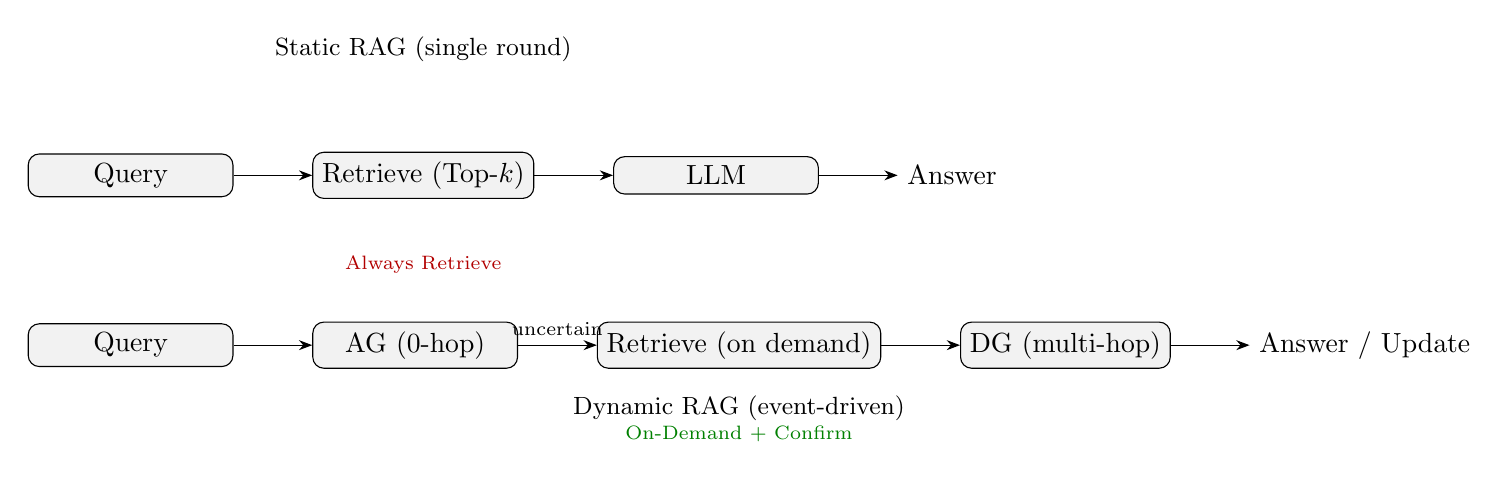
\begin{tikzpicture}[node distance=10mm,>=Stealth,rounded corners]
    % Static pipeline
    \node[draw,fill=gray!10,minimum width=26mm] (q1) {Query};
    \node[draw,fill=gray!10,minimum width=26mm,right=of q1] (r1) {Retrieve (Top-$k$)};
    \node[draw,fill=gray!10,minimum width=26mm,right=of r1] (l1) {LLM};
    \node[right=of l1] (a1) {Answer};
    \draw[->] (q1) -- (r1);
    \draw[->] (r1) -- (l1);
    \draw[->] (l1) -- (a1);
    \node[above of=r1,yshift=6mm,font=\small] {Static RAG (single round)};
    \node[below=6mm of r1,font=\scriptsize,text=red!70!black] {Always Retrieve};
    % Dynamic pipeline
    \node[draw,fill=gray!10,minimum width=26mm,below=16mm of q1] (q2) {Query};
    \node[draw,fill=gray!10,minimum width=26mm,right=of q2] (ag) {AG (0-hop)};
    \node[draw,fill=gray!10,minimum width=26mm,right=of ag] (r2) {Retrieve (on demand)};
    \node[draw,fill=gray!10,minimum width=26mm,right=of r2] (dg) {DG (multi-hop)};
    \node[right=of dg] (a2) {Answer / Update};
    \draw[->] (q2) -- (ag);
    \draw[->] (ag) -- node[above,font=\scriptsize]{uncertain} (r2);
    \draw[->] (r2) -- (dg);
    \draw[->] (dg) -- (a2);
    \node[above of=r2,yshift=-18mm,font=\small] {Dynamic RAG (event-driven)};
    \node[below=6mm of r2,font=\scriptsize,text=green!50!black] {On-Demand + Confirm};
  \end{tikzpicture}
  \caption{Static (single-round) vs dynamic (event-driven) RAG pipelines.
  In dynamic RAG, retrieval happens only under uncertainty (AG), and updates are committed only when DG confirms a gain.}
  \label{fig:static_dynamic_pipeline}
\end{figure}

\begin{table}[H]
  \centering
  \scriptsize
  \begin{tabular}{p{22mm}p{54mm}p{54mm}}
    \toprule
    Aspect & Static RAG (role in this work) & Dynamic RAG (role in this work) \\
    \midrule
    Goal & Measure an \textbf{upper bound on answer / summary quality} under fixed resources & Operationally evaluate \textbf{when to accept} and \textbf{healthiness of updates} over time \\
    Extra processing & None (single pass) & \textbf{AG} triggers on-demand retrieval; \textbf{DG} confirms updates \\
    Metrics & Acc/F1, citation / path faithfulness, P50 & \textbf{Acc/FMR/additional P50} (PSZ), pending$\to$confirmed, temporal consistency \\
    Output & Answer + citations & Answer + \textbf{update log} (AG/DG, F-values, accept / reject) \\
    \bottomrule
  \end{tabular}
  \caption{Static vs dynamic RAG responsibilities (corresponding to \cref{fig:static_dynamic_pipeline}).}
  \label{tab:static_dynamic_responsibility}
\end{table}

\section{Gauge design (theory outline)}\label{sec:gauge_theory}
In this section we sketch how to define normalized differences in edit-path cost and information gain and combine them into the single gauge $\F$ and the two-stage gates; full derivations and extensions (e.g., offline rewiring) are deferred to later sections.

\subsection{Symbol table and premises}\label{sec:graph_model_premise}
\begin{table}[H]
  \centering
  \small
  \begin{tabular}{ll}
    \toprule
    Symbol & Meaning \\
    \midrule
    $\F$ & Unified gauge ($\gednorm - \lambda\,\ignorm$) \\
    $g_0$ & 0-hop evaluation (immediately after tentative wiring) \\
    $g^{(h)}$ & $h$-hop evaluation ($h\in\{1,\dots,H\}$) \\
    $g_{\min}$ & $\min_{1\le h\le H} g^{(h)}$ \\
    $b(t)$ & Operational gauge ($\min\{g_0, g_{\min}\}$) \\
    $\theta_{\mathrm{AG}},\,\theta_{\mathrm{DG}}$ & Quantile-based thresholds (AG/DG) \\
    $\gednorm$ & Normalized edit-path cost (Phase~1 operational GED) \\
    $\ignorm$ & Normalized IG difference ($\Delta H_{\mathrm{norm}}{+}\gamma\,\Delta \mathrm{SP}_{\mathrm{rel}}$) \\
    $c(\cdot)$ & Edit cost function (unit costs for edit operations) \\
    $C_{\mathrm{edit}}$ & Edit-path cost ($\sum c(o)$ over applied edits) \\
    $N_{\mathrm{edit}}$ & Number of edits (for logging) \\
    $S_h$ & $h$-hop induced subgraph \\
    $S_{\mathrm{eval}}$ & Evaluation subgraph (query-centric) \\
    \bottomrule
  \end{tabular}
  \caption{Key symbols and their operational meaning (Phase~1).}
  \label{tab:symbols}
\end{table}

\subsection{Definition of the unified gauge $\F$}
To measure the effect of integrating a new episode, we define \textbf{information consolidation} and \textbf{structural integration}, and bundle them into the single gauge $\F$.

We first define the core of normalized information gain:
\begin{equation}
  \ignorm \;=\; \Delta H_{\mathrm{norm}} \;+\; \gamma\,\Delta \mathrm{SP}_{\mathrm{rel}},
  \qquad \gamma>0.
  \label{eq:ignorm_main}
\end{equation}
\noindent\textit{Note (default parameter).}
In our experiments we set $\gamma{=}1$ by default; sensitivity is reported in the ablation study (see \cref{sec:ablation_analysis}).

\noindent\textit{Interpretation.}
We treat information gain as the combination of \textbf{ordering} (decrease in Shannon entropy) and \textbf{improved path efficiency} (decrease in average shortest-path length).

\noindent\textbf{Short forms and sign conventions.}
For the remainder of the paper we use the shorthand
\[
  \Delta\mathrm{IG}_{\mathrm{norm}}
  \;:=\;
  \Delta H_{\mathrm{norm}} \;+\; \gamma\,\Delta\mathrm{SP}_{\mathrm{rel}},
  \qquad
  \F
  \;=\;
  \gednorm \;-\; \lambda\,\Delta\mathrm{IG}_{\mathrm{norm}}\,,
\]
which is consistent with the shorter form in \cref{eq:F_short_intro}.
We interpret \emph{smaller} $\F$ as \textbf{better} (lower structural cost and stronger information consolidation).
Unless otherwise stated we use the \textbf{normalized} forms
$\gednorm$, $\Delta H_{\mathrm{norm}}$, and $\Delta \mathrm{SP}_{\mathrm{rel}}$.

\paragraph{Design choices (overview)}\label{sec:ig_design_choice}
We favor operational interpretability and therefore define $\Delta\mathrm{IG}$ as a \emph{linear combination of entropy change and path-shortening}.
Alternatives (e.g., ELBO / KL-based objectives), $\gamma$-sweeps, and variants without $\Delta\mathrm{SP}$ are collected as equal-resources ablations in \cref{sec:ablation_analysis}.

Entropy change (ordering / concentration) is defined as a normalized difference:
\begin{equation}
  \Delta H_{\mathrm{norm}}
  \;=\;
  \frac{H_{\text{after}} - H_{\text{before}}}{\log K}.
  \label{eq:dh_norm}
\end{equation}
\noindent\textit{Note (definition of $K$).}
Here $K$ is the number of categories in the \emph{after} set.
Let $S_{\text{base}}$ be a base set (operationally, by default the set of memory candidates; it can be switched to \texttt{pool} / \texttt{link} if needed), and let $q$ be the query episode.
We define
\begin{align*}
  S_{\text{before}} &:= S_{\text{base}},\qquad
  S_{\text{after}}  := S_{\text{base}}\cup\{q\},\quad
  K := |S_{\text{after}}|.
\end{align*}
Each element $i\in S$ is assigned a non-negative weight $w_i\ge 0$ (e.g.\ $w_i=\exp(-d(q,i)/T)$ or $w_i=\exp(\beta\,\cos(q,i))$), and we set $p_i:=w_i/\sum_j w_j$.
Shannon entropy is then
\begin{align*}
  H(S) := -\sum_{i\in S} p_i\,\log p_i,
\end{align*}
with $H_{\text{before}}{=}H(S_{\text{before}})$ and $H_{\text{after}}{=}H(S_{\text{after}})$, and we use $K{=}|S_{\text{after}}|$ for normalization via $\log K$.
In implementation we guard against $K{<}2$ by replacing $\log K$ with $\max\{\log K,\varepsilon\}$ for numerical stability.

\noindent\textit{Note (sign conventions).}
We define $\Delta H_{\mathrm{norm}}$ as \emph{after $-$ before} (so entropy decreases---more order---yield negative values) and $\Delta\mathrm{SP}_{\mathrm{rel}}$ as \emph{before $-$ after} (so path shortening yields positive values).
Information gain is then composed as $\Delta H_{\mathrm{norm}}+\gamma\,\Delta\mathrm{SP}_{\mathrm{rel}}$.
Throughout, each $\Delta(\cdot)$ follows its own sign convention as defined here.

\noindent\textit{Note (stabilizing $\Delta\mathrm{SP}_{\mathrm{rel}}$).}
To guard against very small denominators in average shortest-path length (ASPL), we use
\begin{equation}
  \Delta \mathrm{SP}_{\mathrm{rel}}
  \;=\;
  \frac{L_{\mathrm{before}}-L_{\mathrm{after}}}{\max\{L_{\mathrm{before}},\,\varepsilon\}},
  \label{eq:dsp_rel}
\end{equation}
with default $\varepsilon{=}10^{-8}$.

Structural integration is measured as relative gain in path length:
\begin{equation}
  \Delta \mathrm{SP}
    = \mathrm{SPL}(G')_{\text{after}}-\mathrm{SPL}(G')_{\text{before}},
  \qquad
  \Delta \mathrm{SP}_{\mathrm{rel}}
    = \frac{\mathrm{SPL}(G')_{\text{before}}-\mathrm{SPL}(G')_{\text{after}}}
           {\max\{\mathrm{SPL}(G')_{\text{before}},\,\varepsilon\}},
  \label{eq:dsp_rel_full}
\end{equation}
where $\mathrm{SPL}$ denotes average shortest-path length computed with \textbf{unit edge weights} (all edges of length $1$).
Weighted shortest-path variants are left for future work.


\subsection{0-hop vs multi-hop roles (overview)}
At a high level, 0-hop evaluation $g_0$ is used for \emph{ambiguity detection}: it detects immediate degradation right after tentative wiring.
Multi-hop evaluation, through $g^{(h)}$ and $g_{\min}$, is used for \emph{insight confirmation}: it checks whether structural shortcuts emerge (e.g., shortest-path length decreases) when exploring up to $H$ hops (see minimal examples in the full paper).

\subsection{Gate mechanism (overview)}\label{sec:ag_dg_gate}
The two-stage gate operates as follows.
If $g_0>\theta_{\mathrm{AG}}$, the system deepens exploration (AG).
If $\min\{g_0,g_{\min}\}\le\theta_{\mathrm{DG}}$, the system accepts and commits the update (DG).
Thresholds are calibrated via percentiles on validation data, then fixed for test runs (cf.\ \cref{sec:eval_protocol}).

\section{Evaluation protocol (common)}\label{sec:eval_protocol}
We group conditions that are shared across static and dynamic RAG here; later sections describe only the differences (see also \cref{sec:common_setup} for further details).\footnote{As a first step for reproduction, see the Makefile targets such as \texttt{make exp23-paper}, \texttt{make maze-suite}, and the script \texttt{scripts/codex\_smoke.sh}.}
\begin{itemize}[leftmargin=1.6em]
  \item \textbf{Knowledge source / retrieval / LLM.}
  Corpus, retriever, and generation settings (prompts, temperature, token budgets) are shared across methods.
  \item \textbf{Measurement.}
  We report EM/F1, citation / path faithfulness, and P50 latency.
  For dynamic RAG we additionally report contamination rate (FMR; erroneous acceptances on the update side), PSZ (Acc/FMR/P50 as an SLO-like target), and ZSR (Zero-Search Rate; fraction of 0-hop answers).
  \item \textbf{Equal-resources.}
  Embeddings, ANN index, Top-$k$, LLM, temperature, token budgets, hardware, parallelism, and measurement setup are kept fixed; compressed summaries are tabulated in the appendix.
  \item \textbf{Splits and calibration.}
  We split into train / validation / test; AG/DG thresholds $(\theta_{\mathrm{AG}},\theta_{\mathrm{DG}})$ are calibrated on validation and then fixed for test.
\end{itemize}

\subsection{Maze--RAG embedding correspondence}
We view the maze PoC and the RAG experiments through a shared lens: both operate in an embedding space with local moves, affordances, and outcomes.
Table~\ref{tab:maze_rag_mapping} summarizes the correspondence, including an abstract design layer.
\begin{table}[H]
  \centering
  \scriptsize
  \begin{tabular}{p{20mm}p{36mm}p{40mm}p{34mm}}
    \toprule
    Concept & Maze (PoC) & RAG (this paper) & Abstract (design) \\
    \midrule
    Context & $(x/W,\,y/H)$ & $\varphi(q),\,\varphi(v)$ & Context \\
    Action & $(dx,\,dy)$ & Retrieval / wiring (candidate selection) & Action \\
    Affordance & $\mathrm{wall},\,\mathrm{visits}$ & Similarity, availability / importance & Affordance \\
    Outcome & $\mathrm{success},\,\mathrm{goal}$ & Accept / reject (FMR monitored) & Outcome \\
    Transition (edge) & Neighbors / shortcuts (multi-hop) & Similarity neighborhood $\rightarrow$ wiring ($k$-NN) & Similarity-induced transition \\
    Distance / similarity & Weighted L2 ($\mathbf{w}$) & Cosine similarity & Any $d(\cdot,\cdot)$ satisfying A1--A3 \\
    Embedding & $\mathbf{v}\in\mathbb{R}^8$ & Sentence-BERT $\varphi:\text{text}\to\mathbb{R}^d$ & $\Phi$ \\
    \bottomrule
  \end{tabular}
  \caption{Correspondence between maze and RAG embedding spaces (including an abstract layer).
  While the concrete representations differ, transition definitions and evaluation / control via $\F$ and AG/DG are shared.}
  \label{tab:maze_rag_mapping}
\end{table}

\subsection*{Threats to validity}
\textbf{Internal validity.}
Although we compare methods under equal-resources, we still depend on the choice of grading model and embedding model (Sentence-BERT), as well as on prompt design.
Latency is measured end-to-end (P50) under identical conditions and can be re-measured by rerunning the released scripts (\cref{sec:common_setup}).

\noindent\textbf{External validity.}
Limitations remain in domain coverage, vocabulary, and transfer of HNSW / hop-depth settings across environments.
PSZ should be read as an \emph{SLO}---an operational target---rather than a guarantee of attainability across datasets or infrastructures; we report proximity via the shortfall $s_{\mathrm{PSZ}}$.

The properties of the embedding map $\Phi$ hinted at in \cref{tab:maze_rag_mapping} are made explicit later in \cref{sec:phi_requirements,sec:rag_embed_requirements} as assumptions (A1)--(A3), together with justification for our choice of Sentence-BERT as a representative implementation.

\subsection{Two-phase architecture (awake / sleep)}\label{sec:two_phase_brief}
\textbf{Design intention.}
Edit-path cost EPC is defined as the sum of additive costs for edit operations.
Optimizing it (modulo normalization / upper bounds) is equivalent to pursuing the \textbf{minimum edit distance} $\mathrm{GED}_{\min}$.
Exact computation of $\mathrm{GED}_{\min}$ is in general \textbf{NP-hard} (e.g., \cite{gao2010survey}), and jointly optimizing $\Delta$EPC and $\Delta$IG under sequential updates and real-time constraints is practically difficult.
Thus, \textbf{design choices for real-time operation are unavoidable}.
Rather than separating ``learning'' and ``inference'' into disjoint stages, we adopt a \textbf{two-phase architecture along the time axis}: \textbf{awake (online) vs sleep (offline)}.
In the awake phase (Phase~1), the system processes an input stream with a One-Gauge controller $\F=\gednorm-\lambda\ignorm$ and a two-stage gate (AG for ambiguity, DG for confirmation), making real-time decisions about \textbf{accept / reject / explore / backtrack / memory management}.
In the sleep phase (Phase~2), the system suspends input and performs \textbf{offline optimization for global consistency}: reducing redundancy, rewiring bridges, and compressing the graph (see \cref{sec:phase2_offline} for objectives and implementation considerations).
Figure~\ref{fig:two_phase_overview} illustrates awake / sleep as a \emph{design metaphor}; it is \textbf{not} a claim of physiological equivalence.

\paragraph{Principles for Phase~1 / Phase~2}
The two-phase split is an \textbf{engineering design guideline} motivated by computational efficiency and real-time constraints.
The terms awake / sleep are metaphors inspired by hippocampal forward / reverse replay~\cite{Buzsaki2015,Carr2011}, not claims of biological identity or causality.
In what follows we focus on measurable behavior of $\F$ and on operational predictions; evaluation is grounded in these rather than in neuroscientific claims.

\begin{figure}[H]
  \centering
  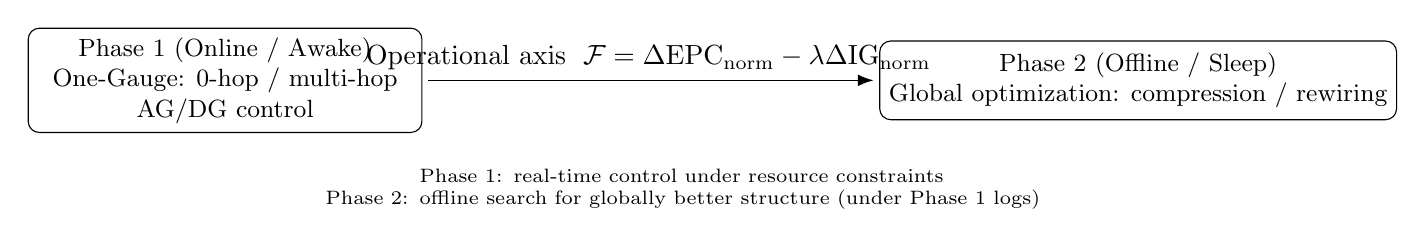
\begin{tikzpicture}[
    node distance=58mm,
    box/.style={rectangle,draw,rounded corners,align=center,minimum width=50mm,minimum height=10mm,font=\small},
    note/.style={align=center,font=\scriptsize,text width=0.8\linewidth},
    >=Latex]
    \node[box] (p1) {Phase 1 (Online / Awake)\\One-Gauge: 0-hop / multi-hop\\AG/DG control};
    \node[box,right=of p1] (p2) {Phase 2 (Offline / Sleep)\\Global optimization: compression / rewiring};
    \draw[->,line width=0.6pt,shorten >=2pt,shorten <=2pt]
      (p1) -- node[above,pos=0.5]{Operational axis $\;\F=\gednorm-\lambda\ignorm\,$} (p2);
    % Central annotation (symmetric placement)
    \path let \p1=(p1), \p2=(p2) in coordinate (mid) at ($ (p1)!0.5!(p2) $);
    \node[note,below=10mm of mid] {Phase~1: real-time control under resource constraints\\Phase~2: offline search for globally better structure (under Phase~1 logs)};
  \end{tikzpicture}
  \caption{Two-phase architecture (awake / sleep) as a design metaphor.
  Phase~1 performs online control with the unified gauge $\F$; Phase~2 performs offline optimization for global structure.}
  \label{fig:two_phase_overview}
\end{figure}

\subsection{Embedding space requirements for $\Phi$}\label{sec:phi_requirements}

The entropy term $\Delta H$ in our gauge is computed from a probability distribution over neighbors in an embedding space $\Phi$ (cf.\ \cref{eq:dh_norm}), and the gauge $\F=\gednorm-\lambda\ignorm$ combines normalized, dimensionless quantities with quantile-based thresholds for the gates (\cref{sec:ag_dg_gate}).
For this combination to behave stably across domains, we impose the following minimal requirements (A1)--(A3) on $\Phi$:
\begin{description}[leftmargin=1.8em,labelwidth=3.5em]
  \item[(A1) Semantic gradient preservation]
  Semantically close episodes should remain close in $\Phi$.
  When this is violated, similarity neighborhoods contain many irrelevant nodes, estimation of $\Delta H$ becomes noisy, and the state distinctions in tables such as \cref{tab:graph_control} deteriorate.
  \item[(A2) Scale normalization]
  Embedding norms should be controlled (e.g., L2-normalized).
  Large norm variations break comparability between the normalized terms $\gednorm$ and $\ignorm$, forcing per-domain retuning of gate thresholds and percentiles.
  While $\Delta\mathrm{SP}_{\mathrm{rel}}$ is computed from unweighted shortest paths on $G'$ and is not directly tied to $\Phi$, induction of $S_h$ (via similarity thresholds / Top-$k$) and any weighted-shortest-path variant benefit from a well-scaled embedding space.
  \item[(A3) Local smoothness]
  Small input changes should induce small changes in $\Phi$.
  Otherwise, paraphrases of an episode can flip $g_0$ or $g_{\min}$ abruptly, causing spiky AG/DG activations and unstable wiring / backtracks.
\end{description}

These requirements are model-agnostic and mainly serve two goals: \textbf{stable estimation of} $\Delta H$ from similarity distributions, and \textbf{consistent scaling} between $\gednorm$ and $\ignorm$.
In the maze PoC, a handcrafted 8-dimensional episode embedding is designed to satisfy (A1)--(A3) via geometric constraints and a monotone mapping of visit counts; in the RAG experiments we use Sentence-BERT~\cite{Reimers2019}, whose contrastive training and unit-norm vectors match these requirements (see \cref{sec:rag_embed_requirements}).

As a lightweight implementation check for (A1)--(A3) we consider:
local Lipschitz tests (bounded variation of similarities under small perturbations), Top-$k$ ranking retention (Jaccard overlap of neighbor sets), and norm concentration ($\|\varphi(x)\|\approx1$ for most $x$).
We compare Sentence-BERT, alternative encoders, and random embeddings under equal-resources and report how $g_0/g_{\min}$, AG/DG rates, and PSZ attainment degrade when these conditions are weakened (\cref{sec:rag_embed_requirements}).

\subsection{Embedding choice for RAG experiments}\label{sec:rag_embed_requirements}

For the RAG experiments we instantiate $\Phi$ with Sentence-BERT~\cite{Reimers2019}.
It provides (i) contrastive training that preserves semantic neighborhoods (A1), (ii) unit-normalized embeddings that satisfy scale constraints (A2), and (iii) empirically smooth responses to paraphrases and small text edits (A3).
We treat these properties as representative rather than unique: other encoders can be plugged in as long as they satisfy the same checks (local Lipschitz behavior, neighbor-set stability, norm concentration).
In the ablations we compare Sentence-BERT, alternative encoders, and randomized embeddings under equal-resources and report the effect on $g_0/g_{\min}$ stability, AG/DG firing rates, PSZ shortfall, and overall RAG performance.

\section{Proof of Concept: partial-observation maze control}\label{sec:maze_experiment}

In this section we treat the maze environment as a small, fully controllable world-model and ask whether a dynamic knowledge graph can use the single gauge $\F$ and the two-stage gate (AG/DG) to \emph{simultaneously} govern (i) selection among new episodes (accept / hold / reject) and (ii) exploitation of the memory graph (explore / backtrack / reuse).
We work with a minimal configuration (8-dimensional state vectors, partial observability, incremental wiring) and examine whether the following design elements operate together as intended:
\begin{enumerate}
  \item \textbf{Unified-gauge control}:
  a single scalar $\F=\gednorm-\lambda\ignorm$ that drives event-based decisions about which candidate edges to commit, defer, or drop, and which branches to explore or prune.
  \item \textbf{Two-stage gate (AG/DG)}:
  0-hop (novelty / ambiguity) detects stagnation and ambiguous local structure; multi-hop evaluation confirms structural shortcuts and triggers backtracking or acceptance when the gauge drops sufficiently.
  \item \textbf{Query-centric multi-hop evaluation}:
  scalable evaluation of EPC and IG on query-centric $k$-hop subgraphs that keeps computations local while still reflecting multi-hop structure.
\end{enumerate}

\paragraph{Role of the PoC}
The maze PoC is primarily a test of \textbf{exploration efficiency} under controlled conditions.
Classical planners such as Dijkstra or A* serve as \emph{reference upper bounds}, not as direct competitors.
The goal is \emph{not} to optimize RAG performance, but to verify that a world-model loop---simultaneously running learning (episode integration) and inference (exploration / backtracking)---behaves as intended when driven by $\F$ and AG/DG.
Concretely, we check:
(i) real-time computability of $\F{=}\gednorm{-}\lambda\Delta\mathrm{IG}$,
(ii) qualitative behavior of the two-stage gate (0-hop stagnation detection, multi-hop shortcut confirmation),
and (iii) scalability and accuracy of query-centric multi-hop evaluation.
The maze-specific state / query / weight design does not carry over to other domains, but the \emph{gauge-and-gate control logic} is reused verbatim in the RAG experiments.

\subsection{Experimental design}

We use grid mazes of sizes $15{\times}15$, $25{\times}25$, and $50{\times}50$ with partial observations (local $3{\times}3$ windows), an episodic memory graph, and query-centric evaluation.
Figure~\ref{fig:maze_overview} shows an example of the PoC setup ($25{\times}25$), including start / goal, visited paths, candidate frontiers, and provisional wiring by the query hub.
The geDIG evaluation combines a Top-$L$ set of provisional edges at 0-hop with stage-wise multi-hop evaluation $g^{(h)}$ and controls commit / hold / rollback via AG/DG.

\begin{figure}[H]
  \centering
  \includegraphics[width=.82\linewidth]{fig4_maze.pdf}
  \caption{Maze PoC overview (example: $25{\times}25$).
  Start / goal, visited paths, candidate frontiers, and query-hub wiring are shown schematically; geDIG evaluates 0-hop provisional links and multi-hop shortcuts with AG/DG control.}
  \label{fig:maze_overview}
\end{figure}

\paragraph{Metrics and success criteria (Maze)}\label{sec:maze_metrics_success}
\textbf{Primary (exploration efficiency)}:
exploration ratio (unique / total), revisit ratio (steps / unique), average backtrack length (AG$\to$DG), dead-end detection delay (dead-end$\to$AG), success rate.
\textbf{Secondary (path quality)}:
Regret $\;=\;$steps$-L^*$ (smaller is better), SPL $=L^*/\max\{L^*,\text{steps}\}$ (closer to $1$ is better).
Diagnostics (reported in the appendix) include runtime P50/P95, AG/DG firing rates, frontier rank correlation between $-\F$ and Dijkstra priority, and path overlap (Jaccard).

As a representative success criterion for 25$\times$25 mazes we target:
exploration ratio $\le0.40$, revisit ratio $\le1.5$, average backtrack length $\le5$, detection delay $\le1$, success rate $\ge95\%$, Regret median $\le{+}3$, SPL mean $\ge0.90$.
Criteria for 15$\times$15 and 50$\times$50 are scaled accordingly.

\begin{table}[H]
  \centering
  \small
  \caption{Representative 25$\times$25 maze results (max steps $=500$, equal-resources).
  geDIG reduces exploration and revisit while keeping success high; full diagnostics (Regret, SPL, AG/DG rates) follow the same pattern as in the Japanese manuscript.}
  \label{tab:maze_25_s500_en}
  % 25x25 maze (500 steps) summary (English version for arXiv v5)
\begin{tabular}{lrr}
\toprule
Metric & Value (eval) & Value (L3) \\ 
\midrule
Success rate & 0.750 & 0.750 \\
Avg. steps & 315.6 & 315.6 \\
Avg. edges & 284.5 & 284.5 \\
AG rate & 1.00 & 0.218 \;\footnotesize(mean over 60 seeds) \\
DG rate & 0.348 & 0.925 \;\footnotesize(mean over 60 seeds) \\
Mean $g_0$ & -0.1618 & -0.1618 \\
Mean $g_{\min}$ & -0.2471 & -0.2471 \\
Avg. eval time (ms) & 4196.6 & 3564.6 \\
P95 eval time (ms) & 30468.7 & 25805.6 \\
\bottomrule
\end{tabular}
\par\noindent\footnotesize Conditions: 25$\times$25 maze, max\_steps=500.\ 
The L3 column reports means over 60 seeds with \texttt{use\_main\_l3=true}; 
the Eval column is taken from the grid experiment (seed=0).\\


\end{table}

\paragraph{Baselines and ablations}
We compare against standard exploration strategies under identical conditions:
Greedy Novelty, $\varepsilon$-greedy, UCB1-like bandit baselines, partially observed A*, and ablations of our own method (EPC-only, IG-only, no AG/DG, 0-hop only).
Dijkstra / A* are used purely as diagnostic upper bounds on structural optimality.

\paragraph{Results (qualitative overview)}
Across seeds and maze sizes, geDIG achieves large reductions in exploration and revisit ratios while maintaining near-immediate dead-end detection.
AG fire rates remain in a moderate band (about 5--10\%), DG fire rates around 2--5\%, and the DG/AG ratio stabilizes near 30--50\%, consistent with the intended division of labor.
Representative 15$\times$15 and 25$\times$25 runs achieve high success rates (around 95--100\% on easier settings, lower on harder 25$\times$25 configurations with tight step budgets), with short backtracks and SPL close to $1$.
Detailed numbers and per-seed plots are provided in the figures and tables shared with the Japanese v5 manuscript and in the public repository.

\section{Experiment II: static RAG baselines}\label{sec:rag_experiment}

\noindent\textit{Recall (short form).}
In this chapter we use the short form of the gauge as well (cf.\ \cref{eq:F_short_intro}).
We focus on the \textbf{pure effect of retrieval and generation} in single-round RAG without updates, under the common conditions described in \cref{sec:eval_protocol,sec:common_setup}.
Here $\F$ is used solely as a \emph{continuous weakening signal inside the retriever}; we \emph{do not} update or rewrite the knowledge graph, and dynamic metrics such as acceptance rate and FMR are reserved for Experiment~III.

\subsection{Common experimental setup (static / dynamic)}\label{sec:common_setup}

Static and dynamic RAG experiments share a common evaluation protocol; differences are localized to their respective sections.
The shared assumptions are:
\begin{itemize}[leftmargin=1.6em]
  \item \textbf{Knowledge source / retriever / LLM.}
  All methods use the same corpus, retriever configuration, and generation model with identical prompts, temperatures, and token budgets.
  \item \textbf{Measurement definitions.}
  We report answer quality (EM/F1; in implementation, token-level overlap is summarized as PER as a surrogate for F1), citation and Path Faithfulness, and latency (measured P50).
  For dynamic RAG we additionally report acceptance rate, FMR (False Merge Rate over accepted events), PSZ (Acc/FMR/P50 SLO) with shortfall $s_{\mathrm{PSZ}}$, and ZSR (Zero-Search Rate; fraction of 0-hop answers with no AG firing).
  \item \textbf{Equal-resource design.}
  The dataset splits, prompts, and inference conditions are defined once here; later chapters only describe their differences.
  Embedder, ANN index, Top-$k$, LLM, temperature, token budgets, hardware, parallelism, and measurement settings are held constant; compressed summaries are tabulated in the appendix.
  \item \textbf{Splits and gate calibration.}
  We split queries into train / validation / test; AG/DG thresholds $(\theta_{\mathrm{AG}},\theta_{\mathrm{DG}})$ are calibrated on validation (via percentiles) and then fixed for test.
\end{itemize}

\subsection{Result summary (static RAG; results-first)}\label{sec:rag_result_summary}

We compare three tiers under equal-resources---flat embedding-based RAG, static graph-based RAG (GNN / Graph Transformer), and \textbf{geDIG-soft reweighting}---and summarize the effect of using $\F=\Delta\mathrm{EPC}_{\mathrm{norm}}-\lambda(\Delta H_{\mathrm{norm}}+\gamma\Delta\mathrm{SP}_{\mathrm{rel}})$ purely on the retrieval side (dynamic metrics are handled in the next chapter).
At a high level:
\begin{itemize}[leftmargin=1.6em]
  \item \textbf{Answer quality (EM/F1 / PER).}
  geDIG (G1) consistently outperforms the strongest static baseline.
  In a representative lite run (500 queries; configuration \texttt{exp23\_paper} in \texttt{experiments/exp2to4\_lite}) static RAG yields EM$\approx0.00$, PER$\approx0.17$, whereas geDIG G1 reaches EM$\approx0.25$, PER$\approx0.42$, i.e., about $+0.25$ absolute improvement in EM.
  \item \textbf{Faithfulness (citations / paths).}
  geDIG improves ``answer-with-correct-citation'' rates and Path Faithfulness while significantly reducing hallucinations (mismatched citations).
  \item \textbf{Latency (P50/P95).}
  Insertion of the weakening step in the retriever keeps P50/P95 latency comparable to static GraphRAG; geDIG operates in the same latency band under the equal-resources constraints.
  \item \textbf{Subgraph quality (Recall@k / IoU / hops).}
  Multi-hop reachability improves while the inclusion of unnecessary nodes (over-exploration) decreases.
\end{itemize}
Informally, the continuous weakening $\sigma(\tau\F)$ allows geDIG to \textbf{keep weak-but-important evidence while filtering noise}.
Detailed scores and distributions are summarized in the tables and figures shared with the Japanese manuscript and reproduced by the public experiment scripts.

\begin{figure}[H]
  \centering
  \includegraphics[width=.74\linewidth]{fig1_rag_performance.pdf}
  \caption{Representative static RAG performance under equal-resources (lite 500-query suite).
  geDIG-soft improves EM / PER and citation faithfulness over the strongest static baseline while keeping latency comparable.}
  \label{fig:rag_static_performance}
\end{figure}

\begin{table}[H]
  \centering
  \small
  \caption{Prompt enrichment and related metrics in static RAG (representative 168-query setting).}
  \label{tab:rag_static_enrichment_en}
  % Auto-generated from resources.md
\begin{tabular}{ll}
\toprule
Key & Value \\ 
\midrule
dataset & experiments/exp2to4\_lite/data/sample\_queries\_500.jsonl \\ 
num\_queries & 500 \\ 
embedding\_model & see YAML: embedding.model \\ 
top\_k & see YAML: retrieval.top\_k \\ 
bm25\_weight & see YAML: retrieval.bm25\_weight \\ 
embedding\_weight & see YAML: retrieval.embedding\_weight \\ 
lambda & see YAML: gedig.lambda \\ 
use\_multihop & see YAML: gedig.use\_multihop \\ 
max\_hops & see YAML: gedig.max\_hops \\ 
theta\_ag & see YAML: gedig.theta\_ag \\ 
theta\_dg & see YAML: gedig.theta\_dg \\ 
\bottomrule
\end{tabular}

\end{table}

\paragraph{Dataset and baselines}
We evaluate three dataset scales---a small 25-query pilot, a 168-query / 20-domain intermediate set, and a main 500-query / 50-domain suite---with a planned extension to 1000+/100+ queries and domains.
Queries mix single-domain, cross-domain, and deeper reasoning questions.
Under equal-resources (same embedder / ANN / token budgets / compute), we compare Static RAG, Frequency-based, Cosine-threshold baselines, GraphRAG~\cite{graphrag2024}, DyG-RAG~\cite{dygrag2024}, KEDKG~\cite{kedkg2024}, and our geDIG variants.
Method-specific best-tuned settings are reserved for supplemental comparisons after the equal-resources runs.

\subsection{Metric definitions and PSZ}

We briefly restate key metrics used in static and dynamic experiments.
PER (Prompt Enhancement Rate) is defined as the ratio of prompt token counts before / after enrichment.
For dynamic RAG we define acceptance and FMR as
\begin{equation}
  \mathrm{Acc} := \frac{\mathrm{TP} + \mathrm{FP}}{N},
  \qquad
  \mathrm{FMR} := \frac{\mathrm{FP}}{\mathrm{TP} + \mathrm{FP}}
  \quad \text{(over accepted events)}.
\end{equation}
Here TP/FP labels come from rule-based grading followed by spot checks by two annotators (with Cohen's $\kappa$ reported); Precision / Recall / F1 are reported alongside, but we keep Acc and FMR conceptually separate to avoid confusion.
Latency metrics track additional processing time (P50/P95/P99 of added latency), and PSZ (Perfect Scaling Zone) is defined as the region
\[
  \mathrm{Acc}\ge95\%,\quad \mathrm{FMR}\le2\%,\quad \mathrm{P50}\le\SI{200}{ms},
\]
with shortfall $s_{\mathrm{PSZ}}$ given by \cref{eq:psz_deficit}.
Table~\ref{tab:key_metrics_direction} summarizes the desired directions on each metric axis; we follow the same conventions in this draft.

\begin{table}[H]
  \centering
  \small
  \caption{Key metrics and desired directions (including PSZ-related targets).}
  \label{tab:key_metrics_direction}
  \begin{tabular}{lll}
    \toprule
    Metric & Definition / meaning & Desired direction \\
    \midrule
    Acceptance (Acc) & Fraction of accepted (TP/FP) updates & $\uparrow$ (target $\ge95\%$) \\
    FMR & False merges among accepted updates & $\downarrow$ (target $\le2\%$) \\
    Additional P50 & Median extra latency (vs static) & $\downarrow$ (target $\le200$\,ms) \\
    Contamination rate $p_{\mathrm{contam}}$ & Fraction of updates later rolled back & $\downarrow$ \\
    Promotion rate & Pending$\to$confirmed transitions & $\uparrow$ \\
    Maze steps & Exploration steps in the PoC & $\downarrow$ \\
    Shortcut contribution $\Delta\mathrm{SP}_{\mathrm{rel}}$ & Relative path-length improvement & $\uparrow$ \\
    \bottomrule
  \end{tabular}
\end{table}

\section{Experiment III: dynamic acceptance (Dynamic GRAG $\times$ geDIG)}

In the dynamic setting, we reuse the same gauge $\F$ and gates but now allow the KG to evolve over time; episodes can be pending, confirmed, or rejected.
The main question is whether, under equal-resources, geDIG can \textbf{reduce contamination and move operating points toward the PSZ band} without incurring prohibitive latency or starving updates.

\paragraph{Summary}
With geDIG-soft applied consistently to retrieval, integration, and summarization (G2), we observe:
improved Temporal Consistency, comparable or lower update lag (ingest$\to$available), reduced KG contamination (FMR), and operating points that move closer to the PSZ region (full attainment is not yet reached).
AG and DG rates remain in controlled bands calibrated on validation, and their time-series traces reveal stable gating behavior even under scale-up.

\paragraph{Dynamic metrics}
Beyond EM/F1 and faithfulness, dynamic runs track:
Temporal Consistency, update lag, rolling FMR, ZSR (0-hop rejection), AG/DG firing rates, and PSZ shortfall $s_{\mathrm{PSZ}}$.
Operating curves sweeping $(\theta_{\mathrm{AG}},\theta_{\mathrm{DG}})$ visualize the trade-offs among Acc, FMR, and latency and highlight reachable regions near PSZ.

\paragraph{Time-series and logs}
We log $\Delta$EPC, $\Delta H$, $\Delta\mathrm{SP}$, and $\F$ together with acceptance decisions (pending$\to$confirmed, confidence values), producing gauge histograms and gating time-series.
These traces make it possible to inspect \emph{when} the system chose to explore, backtrack, or commit, and how often borderline cases were deferred.

\begin{figure}[H]
  \centering
  \includegraphics[width=.78\linewidth]{fig_r_operating_curves.pdf}
  \caption{Example operating curves for dynamic RAG (lite 500-query run).
  Sweeping $(\theta_{\mathrm{AG}},\theta_{\mathrm{DG}})$ traces trade-offs among Acc, FMR, and additional latency; PSZ-compatible regions correspond to low PSZ shortfall $s_{\mathrm{PSZ}}$.}
  \label{fig:dynamic_operating_curves}
\end{figure}

\section{Experiment IV: insight-vector alignment}

We treat DG-confirmed subgraphs as carriers of ``insight vectors'' and test whether simple readouts from these subgraphs align with LLM answer embeddings.
On the 500-query lite run, comparing support vs random controls, we observe a positive shift $\Delta s = s_{\text{support}}-s_{\text{random}}>0$ with strong effect size (Cohen's $d\approx1.0$) and highly significant sign tests ($p\ll0.001$, $N$ in the low hundreds).
Baselines include random subgraphs, Top-$k$ neighborhoods, threshold-based selections, and AG-selected episodes.
These results are preliminary and are not required for the main claims of this paper, but they provide early evidence that DG-confirmed subgraphs encode directions that match the LLM's own answer space.

\section{Ablation analysis and component evaluation}\label{sec:ablation_analysis}

To understand the contribution of each component of $\F$ and of the gating scheme, we conduct equal-resources ablations that remove or vary:
the EPC term, the entropy term $\Delta H$, the path term $\Delta\mathrm{SP}$, the 0-hop / multi-hop split, and the AG/DG gates.
We also sweep $\gamma$ and compare alternative IG definitions (e.g., KL- or ELBO-style objectives) under identical compute and data.

Across maze and RAG settings, we observe:
(i) EPC-only and IG-only variants degrade either structural robustness or information consolidation;
(ii) removing $\Delta\mathrm{SP}$ reduces sensitivity to structural shortcuts and harms multi-hop path quality;
(iii) disabling AG or DG leads to over-exploration, unstable acceptance behavior, or both;
and (iv) moderate variations in $\gamma$ do not qualitatively change behavior within a broad band, but very large or very small values collapse the gauge onto single-term extremes.
These findings support the design choice of combining $\Delta$EPC and $\Delta\mathrm{IG}$ in a single scalar and using a two-stage gate.

\begin{figure}[H]
  \centering
  \includegraphics[width=.78\linewidth]{fig8_ablation.pdf}
  \caption{Representative ablation results (lite 500-query RAG).
  Each component of $\F$ and the AG/DG gates contributes materially: EPC-only and IG-only variants degrade robustness or consolidation, while removing $\Delta\mathrm{SP}$ or gates harms multi-hop path quality and operating points.}
  \label{fig:ablation_overview}
\end{figure}

\section{FEP--MDL bridge (operational proposition)}\label{sec:fep_mdl_bridge}

\noindent\textit{Scope.}
This section provides a heuristic bridge to existing theory; the empirical results and main claims of this paper do not depend on it, and readers may safely skip it on a first pass.

\paragraph{From MDL / FEP to $\F$}
We call an \emph{operational correspondence} any relation that (i) is proportional rather than exact, (ii) has a bounded residual $O(1/N)$ under explicit assumptions, and (iii) yields testable predictions.
Minimum Description Length (MDL) minimizes the sum of model and data code lengths; Free Energy Principle (FEP) treatments minimize a variational free-energy bound on surprise.
Under mild assumptions (normalization, bounded horizon, decomposable edits, stable entropy estimates, and embedding conditions as in \cref{sec:phi_requirements}), we can map these objectives to our gauge via
\[
  \F \;\propto\; \Delta\mathrm{MDL} + O(1/N),
\]
with $\lambda$ acting as a scale-anchoring coefficient roughly analogous to an information temperature.
Table~\ref{tab:theory_mapping_summary} in the Japanese manuscript summarizes structural and information terms in MDL, FEP, and $\F$ side by side.

\paragraph{Implications and limitations}
This correspondence suggests that a single control signal can jointly govern structure edits (EPC) and information consolidation (IG) without double-counting.
The 0-hop vs multi-hop split heuristically mirrors FEP-style error detection vs MDL-style compression.
Ablations in \cref{sec:ablation_analysis} provide empirical support for the roles of $\Delta H$ and $\Delta\mathrm{SP}$, but we do \emph{not} claim formal equivalence to FEP or full MDL optimality; the bridge is intended as an operational guide, not a theorem.

\section{Related work (compressed view)}

We briefly situate geDIG among existing lines of work; a more detailed comparison is given in the Japanese manuscript.
Graph-based RAG systems such as GraphRAG focus on \emph{which paths to retrieve} given a fixed graph, but generally do not provide an explicit, quantitative rule for \emph{when to edit the graph itself}.
Dynamic RAG variants (e.g., DyG-RAG, KEDKG) introduce time-aware and event-driven updates, but again lack a single gauge that unifies structural cost and information gain under equal-resources constraints.
FEP- and MDL-inspired frameworks offer theoretical motivation for compression and free-energy minimization, but typically do not spell out concrete graph-edit rules under realistic compute budgets.

geDIG is designed to sit at the \emph{control layer}: the target of control is the shape of the memory graph (add / rewire / prune), the decision criterion is the single scalar $\F=\gednorm-\lambda\ignorm$, and the operation is split into Phase~1 (online, awake) and Phase~2 (offline, sleep) along the time axis.
In that sense it can be read as a concrete, graph-level implementation of compression principles suggested by MDL, Information Bottleneck, and more recent formulations such as ITI/CEP, while remaining agnostic to the underlying encoder or LLM.

\section{Threats to validity (summary)}

We briefly summarize main threats to validity; the Japanese manuscript contains extended discussion and additional diagnostics.
Internal validity is limited by the choice of grading model, embedder (Sentence-BERT), and prompts; although we use equal-resources comparisons and deterministic scripts, changes in these components could affect absolute numbers.
External validity is limited by domain coverage, vocabulary, and scale: the maze PoC uses synthetic environments, and the RAG experiments use a lite 500-query suite with a single family of LLMs / encoders, so results may not transfer directly to other domains or larger graphs.
Construct validity is constrained by our metric choices: Acc/EM/PER, FMR, PSZ, and ZSR capture important aspects of operation but do not exhaustively describe user-centric utility or long-term safety.
Finally, implementation biases (e.g., particular approximate shortest-path algorithms, embedding approximations) may influence measured $\Delta\mathrm{SP}$ and thereby $\F$; we mitigate this via ablations and by keeping the code and scripts open for inspection and reproduction.

\section{Limitations and future work}\label{sec:limits_future}

This work is explicitly a Phase~1 PoC under constrained compute and dataset size.
Limitations include: modest scale (500-query lite for RAG; limited maze sizes), reliance on a single family of embeddings (Sentence-BERT) and a narrow range of LLMs, simple episode representations, and a focus on short- to mid-range multi-hop reasoning.
Phase~2---offline rewiring under the FEP--MDL bridge, larger graphs, and long-horizon dynamics---is only outlined at a design level (\cref{sec:phase2_offline}).
Extending experiments to public QA benchmarks, diverse domains, and 1M+ node graphs, and running systematic $\lambda$-scans to search for phase-transition-like behavior, remain open for collaboration.

\paragraph{Why PSZ is not yet fully attained (short note)}
In the current dynamic RAG experiments, geDIG reduces PSZ shortfall $s_{\mathrm{PSZ}}$ compared to baselines but does not fully enter the PSZ band.
This is mainly due to conservative hyperparameter choices (single $\lambda$ calibration, percentile-based AG/DG thresholds), limited scale and domain diversity in the lite suites, and gate settings tuned for stability rather than exact PSZ optimality.
We treat PSZ as an SLO-style goal rather than a hard requirement, and expect that larger-scale experiments and more adaptive gating policies can move operating points closer to PSZ without sacrificing robustness.

\section{Phase~2 outlook: offline rewiring}\label{sec:phase2_offline}

Phase~2 is designed as an offline optimization phase that reuses Phase~1 logs to perform global improvements of the knowledge graph.
Conceptually, it targets redundancy reduction, reconstruction of long-range bridges, and compression of over-connected regions, under constraints suggested by the FEP--MDL bridge.
We sketch candidate objectives (e.g., approximate $\mathrm{GED}_{\min}$ under resource constraints, MDL-style description length reductions, preservation of PSZ behavior under replayed traffic) and implementation considerations (incremental APSP / SSSP caches, anytime operation, safe rollback).
A full treatment is left for future work; this section mainly clarifies how Phase~2 is intended to follow Phase~1 in a practical deployment.

\section{Conclusion}

We introduced geDIG, a unified gauge framework for dynamic knowledge graphs that combines normalized edit-path cost and information gain into a single scalar $\F$, and couples it with a two-stage gate (AG/DG).
Across a partial-observation maze PoC and static / dynamic RAG experiments, we showed that this gauge can simultaneously drive exploration, integration, backtracking, and eviction while moving operating points toward a practically useful PSZ region.
Our emphasis has been on operational reproducibility rather than formal optimality: code, scripts, percentile settings, and diagnostics are released so that readers can trace \emph{when} the system worked.
Phase~2 (offline rewiring) and larger-scale studies are intentionally left as open ground for collaboration.

\section*{Acknowledgments}

The author thanks collaborators and early readers for feedback on the Japanese v5 manuscript and on the experiment design, and the broader community for open-source tools and datasets that made this work possible.
Any remaining errors or misinterpretations are the author's responsibility.
We invite collaboration and feedback from the community: this work is conducted by an independent researcher and welcomes reproduction, critical examination, and joint research opportunities on both the theoretical and experimental sides.

\end{document}
